% Options for packages loaded elsewhere
\PassOptionsToPackage{unicode}{hyperref}
\PassOptionsToPackage{hyphens}{url}
\PassOptionsToPackage{dvipsnames,svgnames,x11names}{xcolor}
%
\documentclass[
  letterpaper,
  DIV=11,
  numbers=noendperiod]{scrartcl}

\usepackage{amsmath,amssymb}
\usepackage{iftex}
\ifPDFTeX
  \usepackage[T1]{fontenc}
  \usepackage[utf8]{inputenc}
  \usepackage{textcomp} % provide euro and other symbols
\else % if luatex or xetex
  \usepackage{unicode-math}
  \defaultfontfeatures{Scale=MatchLowercase}
  \defaultfontfeatures[\rmfamily]{Ligatures=TeX,Scale=1}
\fi
\usepackage{lmodern}
\ifPDFTeX\else  
    % xetex/luatex font selection
\fi
% Use upquote if available, for straight quotes in verbatim environments
\IfFileExists{upquote.sty}{\usepackage{upquote}}{}
\IfFileExists{microtype.sty}{% use microtype if available
  \usepackage[]{microtype}
  \UseMicrotypeSet[protrusion]{basicmath} % disable protrusion for tt fonts
}{}
\makeatletter
\@ifundefined{KOMAClassName}{% if non-KOMA class
  \IfFileExists{parskip.sty}{%
    \usepackage{parskip}
  }{% else
    \setlength{\parindent}{0pt}
    \setlength{\parskip}{6pt plus 2pt minus 1pt}}
}{% if KOMA class
  \KOMAoptions{parskip=half}}
\makeatother
\usepackage{xcolor}
\setlength{\emergencystretch}{3em} % prevent overfull lines
\setcounter{secnumdepth}{5}
% Make \paragraph and \subparagraph free-standing
\ifx\paragraph\undefined\else
  \let\oldparagraph\paragraph
  \renewcommand{\paragraph}[1]{\oldparagraph{#1}\mbox{}}
\fi
\ifx\subparagraph\undefined\else
  \let\oldsubparagraph\subparagraph
  \renewcommand{\subparagraph}[1]{\oldsubparagraph{#1}\mbox{}}
\fi


\providecommand{\tightlist}{%
  \setlength{\itemsep}{0pt}\setlength{\parskip}{0pt}}\usepackage{longtable,booktabs,array}
\usepackage{calc} % for calculating minipage widths
% Correct order of tables after \paragraph or \subparagraph
\usepackage{etoolbox}
\makeatletter
\patchcmd\longtable{\par}{\if@noskipsec\mbox{}\fi\par}{}{}
\makeatother
% Allow footnotes in longtable head/foot
\IfFileExists{footnotehyper.sty}{\usepackage{footnotehyper}}{\usepackage{footnote}}
\makesavenoteenv{longtable}
\usepackage{graphicx}
\makeatletter
\def\maxwidth{\ifdim\Gin@nat@width>\linewidth\linewidth\else\Gin@nat@width\fi}
\def\maxheight{\ifdim\Gin@nat@height>\textheight\textheight\else\Gin@nat@height\fi}
\makeatother
% Scale images if necessary, so that they will not overflow the page
% margins by default, and it is still possible to overwrite the defaults
% using explicit options in \includegraphics[width, height, ...]{}
\setkeys{Gin}{width=\maxwidth,height=\maxheight,keepaspectratio}
% Set default figure placement to htbp
\makeatletter
\def\fps@figure{htbp}
\makeatother
% definitions for citeproc citations
\NewDocumentCommand\citeproctext{}{}
\NewDocumentCommand\citeproc{mm}{%
  \begingroup\def\citeproctext{#2}\cite{#1}\endgroup}
\makeatletter
 % allow citations to break across lines
 \let\@cite@ofmt\@firstofone
 % avoid brackets around text for \cite:
 \def\@biblabel#1{}
 \def\@cite#1#2{{#1\if@tempswa , #2\fi}}
\makeatother
\newlength{\cslhangindent}
\setlength{\cslhangindent}{1.5em}
\newlength{\csllabelwidth}
\setlength{\csllabelwidth}{3em}
\newenvironment{CSLReferences}[2] % #1 hanging-indent, #2 entry-spacing
 {\begin{list}{}{%
  \setlength{\itemindent}{0pt}
  \setlength{\leftmargin}{0pt}
  \setlength{\parsep}{0pt}
  % turn on hanging indent if param 1 is 1
  \ifodd #1
   \setlength{\leftmargin}{\cslhangindent}
   \setlength{\itemindent}{-1\cslhangindent}
  \fi
  % set entry spacing
  \setlength{\itemsep}{#2\baselineskip}}}
 {\end{list}}
\usepackage{calc}
\newcommand{\CSLBlock}[1]{\hfill\break\parbox[t]{\linewidth}{\strut\ignorespaces#1\strut}}
\newcommand{\CSLLeftMargin}[1]{\parbox[t]{\csllabelwidth}{\strut#1\strut}}
\newcommand{\CSLRightInline}[1]{\parbox[t]{\linewidth - \csllabelwidth}{\strut#1\strut}}
\newcommand{\CSLIndent}[1]{\hspace{\cslhangindent}#1}

\KOMAoption{captions}{tableheading}
\makeatletter
\@ifpackageloaded{caption}{}{\usepackage{caption}}
\AtBeginDocument{%
\ifdefined\contentsname
  \renewcommand*\contentsname{Table of contents}
\else
  \newcommand\contentsname{Table of contents}
\fi
\ifdefined\listfigurename
  \renewcommand*\listfigurename{List of Figures}
\else
  \newcommand\listfigurename{List of Figures}
\fi
\ifdefined\listtablename
  \renewcommand*\listtablename{List of Tables}
\else
  \newcommand\listtablename{List of Tables}
\fi
\ifdefined\figurename
  \renewcommand*\figurename{Figure}
\else
  \newcommand\figurename{Figure}
\fi
\ifdefined\tablename
  \renewcommand*\tablename{Table}
\else
  \newcommand\tablename{Table}
\fi
}
\@ifpackageloaded{float}{}{\usepackage{float}}
\floatstyle{ruled}
\@ifundefined{c@chapter}{\newfloat{codelisting}{h}{lop}}{\newfloat{codelisting}{h}{lop}[chapter]}
\floatname{codelisting}{Listing}
\newcommand*\listoflistings{\listof{codelisting}{List of Listings}}
\makeatother
\makeatletter
\makeatother
\makeatletter
\@ifpackageloaded{caption}{}{\usepackage{caption}}
\@ifpackageloaded{subcaption}{}{\usepackage{subcaption}}
\makeatother
\ifLuaTeX
  \usepackage{selnolig}  % disable illegal ligatures
\fi
\usepackage{bookmark}

\IfFileExists{xurl.sty}{\usepackage{xurl}}{} % add URL line breaks if available
\urlstyle{same} % disable monospaced font for URLs
\hypersetup{
  pdftitle={Note intermédiaire rapport de stage},
  pdfauthor={Mathieu Thomassin},
  pdfkeywords={machine learning, deep learning,
cybersécurité, Earthquakes},
  colorlinks=true,
  linkcolor={blue},
  filecolor={Maroon},
  citecolor={Blue},
  urlcolor={Blue},
  pdfcreator={LaTeX via pandoc}}

\title{Note intermédiaire rapport de stage}
\author{Mathieu Thomassin}
\date{2024-05-28}

\begin{document}
\maketitle
\begin{abstract}
L'Insee a renforcé récemment ses capacités opérationnelles en terme de
cybersécurité via notamment la création de son SOC (Security Operation
Center) en septembre 2023. Devant la quantité de données et leur
diversité et face aux évolutions des techniques et tactiques des
attaquants, les méthodes de détection de cyberattaques peuvent avoir des
limites. L'application d'algorithmes de Machine Learning peut aider les
analystes SOC à repérer des attaques. Se déroulant au sein de l'équipe
SOC construite depuis peu, le stage va permettre d'appliquer des
techniques de Machine Learning et de deep learning sur des jeux de
données réelles, afin de participer à la détection d'incidents de
sécurité.
\end{abstract}

\renewcommand*\contentsname{Table of contents}
{
\hypersetup{linkcolor=}
\setcounter{tocdepth}{3}
\tableofcontents
}
\section{Introduction}\label{introduction}

\begin{itemize}
\tightlist
\item
  \textbf{Présentation du stagiaire et du maître de stage} :

  \begin{itemize}
  \tightlist
  \item
    stagiaire: Mathieu THOMASSIN
  \item
    maître de stage: Michael ORSUCCI
  \item
    Titre du stage: Machine Learning appliqué à la cybersécurité
  \end{itemize}
\end{itemize}

\section{Description de la mission}\label{description-de-la-mission}

\subsection{Environnement de travail:}\label{environnement-de-travail}

\begin{itemize}
\item
  \textbf{Présentation de l'organisation} : L'Insee a renforcé récemment
  ses capacités opérationnelles en terme de cybersécurité via notamment
  la création de son SOC (Security Operation Center) en septembre 2023.
  Cette équipe est répartie entre les sites de la DR de Nantes et la DR
  de Metz et a pour objectif de renforcer la sécurité du SI.
\item
  \textbf{Contexte général du stage} : Devant la quantité de données et
  leur diversité et face aux évolutions des techniques et tactiques des
  attaquants, les méthodes de détection de cyberattaques peuvent avoir
  des limites. L'application d'algorithmes de Machine Learning peut
  aider les analystes SOC à repérer des attaques. Le stage va permettre
  d'appliquer des techniques de Machine Learning et de deep learning sur
  des jeux de données réelles, afin de participer à la détection
  d'incidents de sécurité.
\item
  \textbf{Objectifs du Stage} :

  \begin{itemize}
  \tightlist
  \item
    Objectifs principaux: l s'agit d'appliquer des techniques de
    détection de requêtes malveillantes arrivant dans le SI de l'Insee.
    Les requêtes arrivant au sein du SI peuvent être centralisées par un
    SIEM (Security information and event management).
  \item
    Résultats attendus:

    \begin{itemize}
    \tightlist
    \item
      Offrir un service s'ajoutant au SIEM permettant d'identifier des
      requêtes malveillantes.
    \item
      Pouvoir comparer différents \emph{meilleurs} modèles (au sens
      d'une recherche dans les hyper paramètres) entre eux
    \item
      Favoriser les bonnes pratiques du MLOps: reproductibilité,
      contrôle de version, automatisation, surveillance, collaboration
    \item
      Étendre la méthodologie à des jeux de données publics différents
    \item
      Explorer les algorithmes de détection d'anomalie
    \end{itemize}
  \end{itemize}
\item
  \textbf{Enjeux} :

  \begin{itemize}
  \tightlist
  \item
    Importance de la mission pour l'entreprise: à titre d'exemple,
    l'Insee détient l'application Elire. Une attaque réussie sur cette
    application perturberait le bon déroulement de la vie démocratique.
  \item
    Impact potentiel des résultats: La détection de requêtes
    malveillantes pourrait permettre de déjouer une attaque en cours
  \end{itemize}
\end{itemize}

\paragraph{3. Timing Prévisionnel}\label{timing-pruxe9visionnel}

\begin{itemize}
\tightlist
\item
  \textbf{Calendrier des Étapes} :

  \begin{itemize}
  \tightlist
  \item
    Détail du planning prévisionnel des différentes phases du projet
    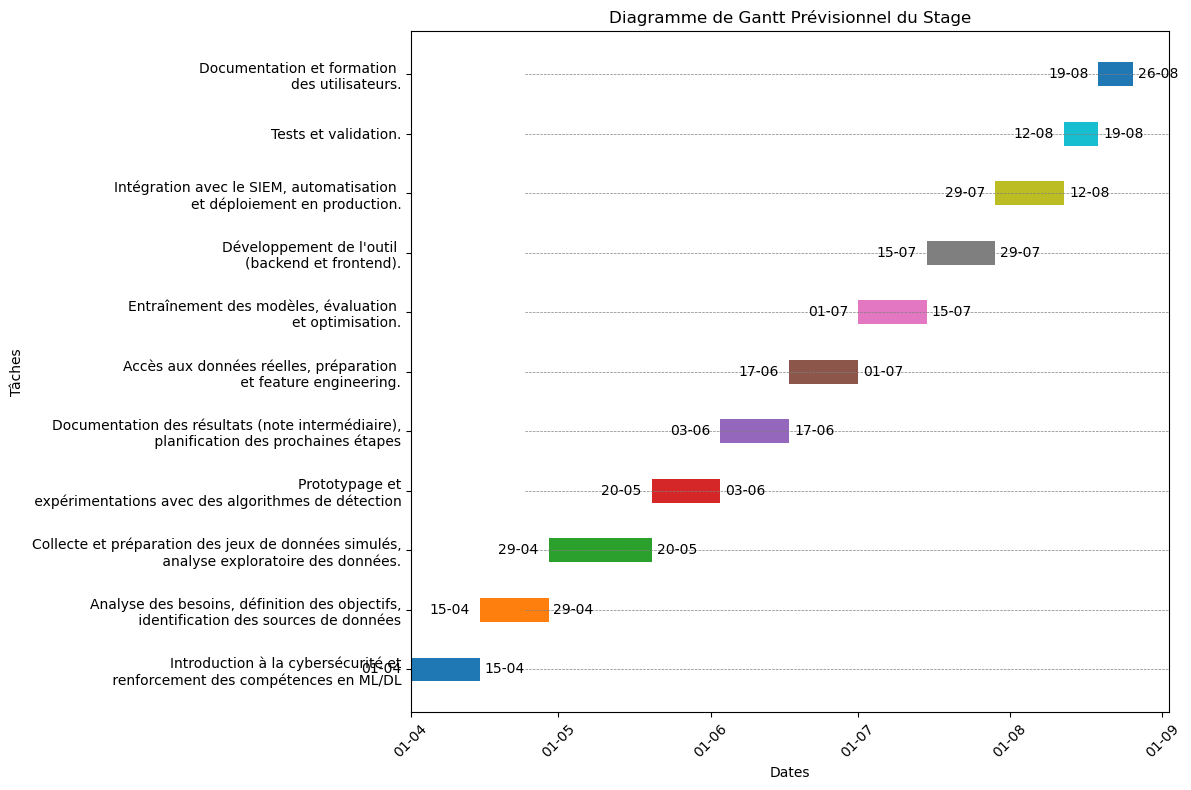
\includegraphics{images/gantt_prevision.png}
  \item
    Échéances importantes et jalons:

    \begin{itemize}
    \tightlist
    \item
      note intermédiaire (1er juin)
    \item
      être prêt pour tester pendant les élections européennes (8 et 9
      juin)
    \item
      surveillance pendant les jeux olympiques (26 juillet au 11 août)
    \item
      rapport final (fin août)
    \end{itemize}
  \end{itemize}
\end{itemize}

\begin{itemize}
\tightlist
\item
  \textbf{Avancement Actuel} :

  \begin{itemize}
  \item
    Comparaison avec le calendrier initial:
    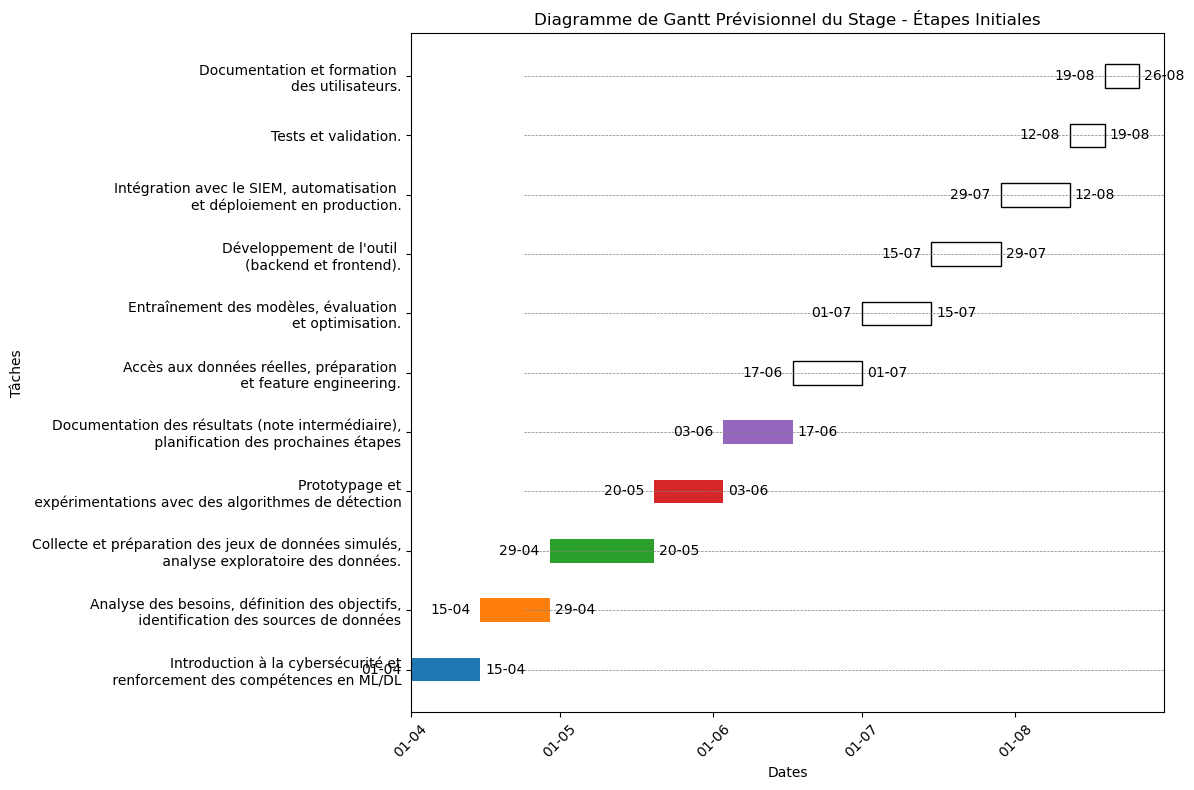
\includegraphics{images/gantt_realise.png}
  \item
    Retards éventuels et raisons:

    \begin{itemize}
    \tightlist
    \item
      Les premiers tests et expérimentations ont eu lieu, cependant,
      j'ai préféré commencer à comprendre plus en profondeur les design
      patterns de deep learning ainsi que le fonctionnement de MLFlow
      avant de pousser davantage la comparaison des modèles et des
      datasets. MLFLow va permettre une bonne méthode de comparaison et
      de sélection des meilleurs modèles, dans la perspective d'une
      intégration avec une mise en production.
    \end{itemize}

    Je n'utilise donc pour le moment qu'un seul dataset constitué de
    bonnes et mauvaises requêtes labellisées, un seul modèle (sur
    plusieurs déjà entraînés).

    Je n'ai pas encore terminé l'intégration sur MLFlow.
  \end{itemize}
\end{itemize}

\paragraph{4. Méthodologies Utilisées et
Prévisionnelles}\label{muxe9thodologies-utilisuxe9es-et-pruxe9visionnelles}

\begin{itemize}
\tightlist
\item
  \textbf{Collecte de Données} :

  \begin{itemize}
  \tightlist
  \item
    Sources des données:

    \begin{itemize}
    \tightlist
    \item
      dataset public pour l'entraînement des modèles:

      \begin{itemize}
      \tightlist
      \item
        http://www.secrepo.com/\#
      \item
        https://www.netresec.com/index.ashx?page=PcapFiles
      \item
        https://www.stratosphereips.org/datasets-overview
      \item
        \href{https://medium.com/@dylan.d.zheng/}{description des
        datasets}
      \item
        datasets-for-network-security-e25238704c7f
      \item
        \href{https://github.com/jivoi/awesome-ml-for-cybersecurity?tab=readme-ov-file}{dépôt
        github contenant des liens vers plusieurs datasets}
      \item
        \href{https://github.com/faizann24/Fwaf-Machine-Learning-driven-Web-Application-Firewall/tree/master}{Good
        et Bad queries dataset}
      \end{itemize}
    \item
      données issues du SIEM, soit le POC en cours (fin mai) soit
      potentiellement le SIEM qui sera mis en place
    \end{itemize}
  \item
    Méthodes de collecte:

    \begin{itemize}
    \tightlist
    \item
      téléchargement à partir des liens
    \item
      téléchargement au format Json à partir d'une recherche dans
      Splunk. Il serait souhaitable de réussir à utiliser l'API du SIEM
      afin d'automatiser cette tâche et de reproduire les résultats.
    \end{itemize}
  \end{itemize}
\end{itemize}

\begin{itemize}
\tightlist
\item
  \textbf{Préparation et Nettoyage des Données} :

  \begin{itemize}
  \item
    Techniques de nettoyage: \textbf{Lecture des fichiers de requêtes},
    étiquetage en fonction de leur nature (bonne ou mauvaise) et
    concaténation dans un DataFrame.

    \textbf{Étiquetage des données} : - Les données sont lues à partir
    de fichiers texte et chaque ligne est étiquetée comme étant soit une
    mauvaise requête (1) soit une bonne requête (0)

    \textbf{Séparation des ensembles d'entraînement et de test} :

    \begin{itemize}
    \tightlist
    \item
      Les données étiquetées sont divisées en deux ensembles : un
      ensemble d'entraînement (80\%) et un ensemble de test (20\%).
    \end{itemize}

    \textbf{Tokenisation personnalisée} :

    \begin{itemize}
    \tightlist
    \item
      Une fonction de tokenisation personnalisée utilise des expressions
      régulières pour extraire des tokens pertinents des textes, y
      compris les mots, les chiffres, les URL et certains caractères
      spéciaux.
    \end{itemize}

    \textbf{Vectorisation TF-IDF} :

    \begin{itemize}
    \tightlist
    \item
      Les données textuelles sont transformées en matrices de
      caractéristiques en utilisant la vectorisation TF-IDF, ce qui
      permet de préparer les données pour un modèle de machine learning.
    \end{itemize}
  \item
    Outils utilisés:

    \begin{itemize}
    \tightlist
    \item
      \textbf{Pandas} : Manipulation de données.
    \item
      \textbf{Scikit-learn (sklearn)} :

      \begin{itemize}
      \tightlist
      \item
        \texttt{train\_test\_split} : Séparation des données en
        ensembles d'entraînement et de test.
      \item
        \texttt{TfidfVectorizer} : Vectorisation des données textuelles
        en utilisant TF-IDF.
      \end{itemize}
    \item
      \textbf{re} : Utilisation d'expressions régulières pour la
      tokenisation personnalisée.
    \end{itemize}
  \end{itemize}
\item
  \textbf{Analyse et Modélisation} :

  \begin{itemize}
  \tightlist
  \item
    Méthodes d'analyse (exploratoire, descriptive): \textbf{Extraction
    des caractéristiques} :

    \begin{itemize}
    \tightlist
    \item
      Une fonction \texttt{extract\_features} est définie pour extraire
      les parties importantes des requêtes, en particulier les noms de
      scripts ou de fichiers ciblés.
    \item
      Les données sont nettoyées pour éliminer les caractères non
      désirés et les retours à la ligne, puis les scripts/fichiers sont
      extraits et ajoutés dans une nouvelle colonne \texttt{Script} du
      DataFrame. \textbf{Statistiques descriptives} :
    \item
      Les statistiques descriptives sur les scripts/fichiers ciblés sont
      générées en utilisant \texttt{value\_counts()} pour obtenir la
      fréquence des différents scripts/fichiers ciblés.
    \item
      \href{images/Fréquence\%20des\%20fichiers\%20scripts\%20ciblés.png}{Les
      20 scripts/fichiers les plus fréquents sont affichés.}
    \end{itemize}
  \item
    Modèles de machine learning ou autres techniques analytiques
    envisagées
  \end{itemize}
\item
  \textbf{Évaluation des Modèles} :

  \begin{itemize}
  \tightlist
  \item
    Métriques de performance prévues
  \item
    Stratégies de validation
  \end{itemize}
\end{itemize}

\paragraph{5. État des Travaux}\label{uxe9tat-des-travaux}

\begin{itemize}
\tightlist
\item
  \textbf{Travaux Réalisés Jusqu'à Présent} :

  \begin{itemize}
  \tightlist
  \item
    Progrès réalisés
  \item
    Résultats obtenus jusqu'ici
  \end{itemize}
\item
  \textbf{Difficultés Rencontrées} :

  \begin{itemize}
  \tightlist
  \item
    Problèmes techniques ou méthodologiques
  \item
    Solutions envisagées ou mises en place
  \end{itemize}
\item
  \textbf{Travaux Restants} :

  \begin{itemize}
  \tightlist
  \item
    Étapes à venir
  \item
    Objectifs pour les prochaines semaines
  \end{itemize}
\end{itemize}

\paragraph{6. Bibliographie}\label{bibliographie}

Le SOC étant une nouvelle unité, il n'y a pas eu de travaux sur le sujet
en amont. J'ai axé ma recherche bibliographique autour des techniques de
machine learning pour la cybersécurité, et autour des techniques de Deep
Learning.

\begin{itemize}
\tightlist
\item
  \textbf{Références Utilisées} :

  \begin{itemize}
  \tightlist
  \item
    Articles scientifiques:

    \begin{itemize}
    \tightlist
    \item
      Isolation Forest, Liu, Ting, Zhou
    \item
      R. Fontugne, P. Borgnat, P. Abry, K. Fukuda. ``MAWILab: Combining
      diverse anomaly detectors for automated anomaly labeling and
      performance benchmarking''. ACM CoNEXT 2010. Philadelphia, PA.
      December 2010.
    \end{itemize}
  \item
    Livres et manuels:

    \begin{itemize}
    \tightlist
    \item
      An introduction to statistical learning with applications in
      Python
    \item
      Deep Learning Patterns and Practices, Andrew Ferlitsch
    \item
      Deep Learning from Scratch - Building with Python from first
      principles, Seth Weidman
    \item
      Deep Learning\_ A Visual Approach -- Andrew Glassner --
      Illustrated, 2021
    \item
      Machine learning with Python cookbook, Kyle Gallatin \& Chris
      Albon
    \item
      Deep Learning, Ian Goodfellow
    \item
      Machine Learning for cybersecurity, Emmanuel Tsukerman, (Chapter 6
      Automatic Intrusion Detection)
    \item
      Machine Learning for computer and Cyber Security, Principles,
      Algorithms, and Practices, Brij B. Gupta
    \end{itemize}
  \item
    Documentation technique
  \end{itemize}
\item
  \textbf{Ressources Additionnelles} :

  \begin{itemize}
  \tightlist
  \item
    Sites web

    \begin{itemize}
    \tightlist
    \item
      \href{https://scikit-learn.org/stable/user_guide.html\#user-guide}{Scikit-Learn}
    \end{itemize}
  \item
    Outils et bibliothèques spécifiques

    \begin{itemize}
    \tightlist
    \item
      \href{https://www.splunk.com/fr_fr}{Splunk}
    \end{itemize}
  \end{itemize}
\item
  Articles:
\end{itemize}

\paragraph{7. Conclusion}\label{conclusion}

\begin{itemize}
\tightlist
\item
  \textbf{Synthèse de l'Avancement} :

  \begin{itemize}
  \tightlist
  \item
    Résumé des principales réalisations
  \item
    Confirmation du bon déroulement du stage
  \end{itemize}
\item
  \textbf{Perspectives} :

  \begin{itemize}
  \tightlist
  \item
    Étapes finales du stage
  \item
    Objectifs pour la phase suivante
  \end{itemize}
\end{itemize}

\subsubsection{Format et Soumission}\label{format-et-soumission}

\begin{itemize}
\tightlist
\item
  \textbf{Format du Document} :

  \begin{itemize}
  \tightlist
  \item
    Nommer le fichier suivant le format : « NOM\_Prénom\_mi\_parcours »
  \end{itemize}
\item
  \textbf{Modes de Soumission} :

  \begin{itemize}
  \tightlist
  \item
    Soumission sur Moodle
  \item
    Envoi par mail à l'enseignant référent
  \end{itemize}
\end{itemize}

En suivant ce plan, vous devriez être en mesure de rédiger une note
d'étape complète et structurée, respectant les exigences de votre
programme de stage. Assurez-vous de respecter la longueur recommandée (2
à 3 pages) en étant concis et précis dans vos descriptions.

\subsubsection{2. État de l'Art}\label{uxe9tat-de-lart}

\begin{itemize}
\tightlist
\item
  \textbf{Revue de Littérature} : Synthèse des travaux précédents,
  articles scientifiques, et technologies utilisées en lien avec la
  problématique du stage.
\end{itemize}

Le SOC étant une nouvelle unité, il n'y a pas eu de travaux sur le sujet
en amont. J'ai axé ma recherche bibliographique autour des techniques de
machine learning pour la cybersécurité, et autour des techniques de Deep
Learning.

\begin{itemize}
\tightlist
\item
  Livres:

  \begin{itemize}
  \tightlist
  \item
    An introduction to statistical learning with applications in Python
  \item
    Deep Learning Patterns and Practices, Andrew Ferlitsch
  \item
    Deep Learning from Scratch - Building with Python from first
    principles, Seth Weidman
  \item
    Deep Learning\_ A Visual Approach -- Andrew Glassner -- Illustrated,
    2021
  \item
    Machine learning with Python cookbook, Kyle Gallatin \& Chris Albon
  \item
    Deep Learning, Ian Goodfellow
  \item
    Machine Learning for cybersecurity, Emmanuel Tsukerman, (Chapter 6
    Automatic Intrusion Detection)
  \item
    Machine Learning for computer and Cyber Security, Principles,
    Algorithms, and Practices, Brij B. Gupta
  \end{itemize}
\item
  Articles:

  \begin{itemize}
  \item
    Isolation Forest, Liu, Ting, Zhou
  \item
    R. Fontugne, P. Borgnat, P. Abry, K. Fukuda. ``MAWILab: Combining
    diverse anomaly detectors for automated anomaly labeling and
    performance benchmarking''. ACM CoNEXT 2010. Philadelphia, PA.
    December 2010.
  \item
    \textbf{Technologies et Outils} : Présentation des technologies,
    outils, et bibliothèques couramment utilisés en data science et
    spécifiques au projet.
  \end{itemize}
\end{itemize}

Pour ce projet, j'utilise Python, et des notebook Jupyter, au sein
d'environnement hébergés sur la plateforme Onyxia (qui met à dispositio
un GPU) ou son équivalent en interne à l'Insee (qui n'en dispose pas).
J'utilise les packages classiques de machine learning dont scikit-learn,
et les outils associés: TfidfVectorizer, tensorflow,
LogisticRegressionLSTM, XGBoost CNN, KFold GridSearchCV. J'ai également
commencé à utiliser l'outil MLFlow, qui est une plateforme permettant de
gére le cycle de vie d'un projet de machine learning de bout en bout,
notamment les étapes d'expérimentation et d'amélioration continue.

\begin{figure}[H]

{\centering 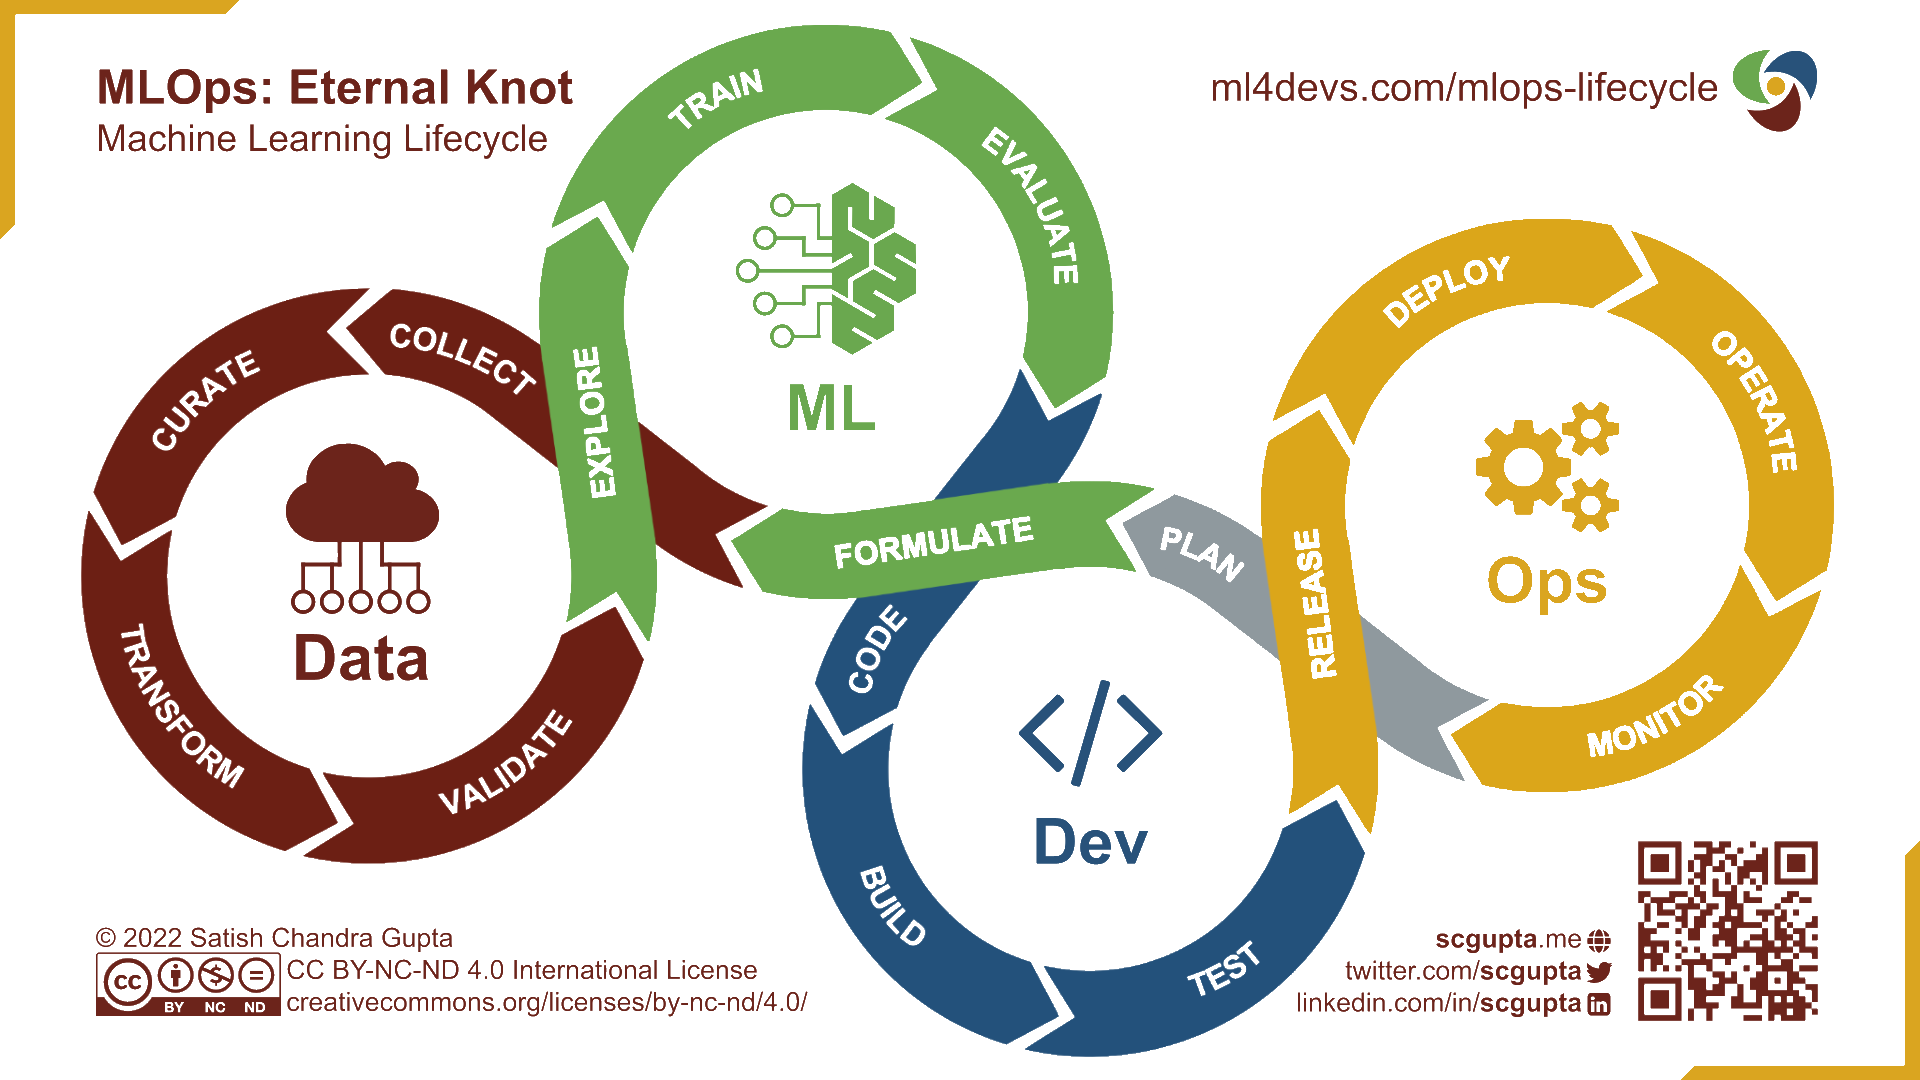
\includegraphics{images/mlops.png}

}

\caption{L'approche MLOps}

\end{figure}%

\subsubsection{3. Méthodologie}\label{muxe9thodologie}

\begin{itemize}
\tightlist
\item
  \textbf{Collecte de Données} : Sources des données, méthodes de
  collecte, et description des jeux de données utilisés.
\end{itemize}

Les données se classent en deux catégories: les données sur lesquelles
les modèles sont entraînés, et les données issues de Splunk. Pour le
moment, j'ai testé différents algorithmes sur un unique jeu de données
que je nomme {[}``Good-Bad
queries''{]}\url{https://github.com/faizann24/Fwaf-Machine-Learning-driven-Web-Application-Firewall.git}

\begin{itemize}
\tightlist
\item
  \textbf{Préparation des Données} : Techniques de nettoyage,
  transformation, et enrichissement des données.
\item
  \textbf{Exploration des Données} : Analyse exploratoire,
  visualisations, et insights préliminaires obtenus des données.
\item
  \textbf{Modélisation} : Description des modèles de machine learning ou
  autres techniques analytiques utilisés. Justification des choix de
  modèles.
\item
  \textbf{Évaluation des Modèles} : Métriques et méthodes utilisées pour
  évaluer la performance des modèles.
\end{itemize}

\subsubsection{4. Développement et
Implémentation}\label{duxe9veloppement-et-impluxe9mentation}

\begin{itemize}
\tightlist
\item
  \textbf{Architecture du Système} : Schéma et description de
  l'architecture du système ou de la solution développée.
\item
  \textbf{Pipeline de Données} : Description du pipeline de traitement
  des données, de l'ingestion à l'analyse.
\item
  \textbf{Déploiement} : Processus de déploiement des modèles ou
  solutions, environnements utilisés (local, cloud, etc.), et outils de
  déploiement.
\end{itemize}

\subsubsection{5. Résultats et
Discussions}\label{ruxe9sultats-et-discussions}

\begin{itemize}
\tightlist
\item
  \textbf{Résultats Obtenus} : Présentation des résultats des analyses
  et des performances des modèles.
\item
  \textbf{Interprétation des Résultats} : Analyse et interprétation des
  résultats. Comparaison avec les attentes initiales et les benchmarks.
\item
  \textbf{Limites et Contraintes} : Discussion sur les limites
  rencontrées, les défis techniques, et les contraintes liées aux
  données ou aux outils.
\end{itemize}

\subsubsection{6. Conclusion et
Perspectives}\label{conclusion-et-perspectives}

\begin{itemize}
\tightlist
\item
  \textbf{Synthèse du Travail} : Résumé des principales réalisations et
  des contributions du stage.
\item
  \textbf{Perspectives d'Avenir} : Suggestions pour des travaux futurs,
  améliorations possibles, et nouvelles pistes de recherche ou de
  développement.
\end{itemize}

\subsubsection{7. Références}\label{ruxe9fuxe9rences}

\begin{itemize}
\tightlist
\item
  \textbf{Bibliographie} : Liste des ouvrages, articles, et ressources
  consultés pour la réalisation du projet.
\item
  \textbf{Outils et Logiciels} : Références des outils et logiciels
  utilisés.
\end{itemize}

\subsubsection{8. Annexes}\label{annexes}

\begin{itemize}
\tightlist
\item
  \textbf{Code Source} : Extraits de code pertinents ou lien vers un
  dépôt de code.
\item
  \textbf{Documents Supplémentaires} : Diagrammes, schémas, documents
  techniques, etc.
\end{itemize}

Ce plan vous fournira une structure claire et organisée pour votre note
intermédiaire, couvrant tous les aspects essentiels de votre stage en
data science. Chaque section peut être adaptée en fonction des
spécificités de votre projet et des exigences de votre programme de
master.

\subsection{Introduction}\label{introduction-1}

Based on data up to and including 1971, eruptions on La Palma happen
every 79.8 years on average.

\subsection{Data \& Methods}\label{sec-data-methods}

\subsection{Conclusion}\label{conclusion-1}

\subsection*{References}\label{references}
\addcontentsline{toc}{subsection}{References}

\phantomsection\label{refs}
\begin{CSLReferences}{0}{1}
\end{CSLReferences}



\end{document}
